\chapter{Introduction}
The direct numerical simulation (DNS) of the Navier-Stokes equations is a mathematical tool used to analyze turbulent flows since it allows to have an inner viewpoint in the transition and turbulence phenomena processes. It is part of the so called Computation Fluid Dynamics, or CFD, research field. 
Given the high computational cost of these simulations, DNS is not used to reproduce real-life flows, but as a research tool for flows with simple boundaries\cite{dns:tool}. \par
Despite of such kind of simulations, due to its limits, could seems useless, they assume relevant importance in the study of the turbulence, who, dominating the small scales, affect the behavior of the large scales, determining the raise of phenomenas such as flow separations, drag increases or losses of lift.
These simulations rely on high accuracy computational methods and they do not employ turbulence models, hence they require an ever-increasing computational power, as we move towards engineering relevant Reynolds numbers.
\par
In this chapter we will provide a briefly description of the phenomena, then we will recall the main statistical quantities used to characterize turbulent flows. In the second chapter we will describe the geometry of the domain along with the governing equations for the problem presented, the structure of the code, discretization, domain decomposition and I/O.
The third chapter will deal with code benchmarks while the fourth will show the results of our simulation. Finally we will draw a line of possible future works.

\section{Turbulent flows}
Every smoker can observe the nature of turbulence one inch away from their nose.
However a proper definition of turbulence is not yet given, due to the complexity of turbulence behaviour. \par
To use Prandtl words, who began an important lecture as follows: \\~\\
\emph{``What I am about to say on the phenomena of turbulent flows is still far from conclusive. It concerns, rather, the first steps in a new path which I hope will be followed by many others. The researches on the problem of turbulence which have been carried on at G\"{o}ttingen for about five years have unfortunately left the hope of thorough understanding of turbulent flow very small. The photographs and kinetographic pictures have shown us only how hopelessly complicated this flow is.''} \\~\\

Nowadays we can entrust to computational units that allows us to be no longer \emph{``hopeless''} as Prandtl was, although we are still far from having a solution, or at least a unique definition, of what the turbulence is. 
At the present time we define the turbulence as a flow regime, characterized by high Reynolds numbers and the presence of high level of diffusivity and irregularity, dissipation and three dimensional chaotic fluctuations in space and time\cite{turbulence:def}.

\section{General concepts}
An elderly definition of turbulence was provided by Hinze~\cite{Hinze}, in 1959, and say:\\~\\
\emph{``Turbulent fluid motion is an irregular condition of flow in which the various quantities show a random variation with time and space coordinates, so that statistically distinct average values can be discerned''}.\\~\\
The concept of \emph{average} is the keyword that humanity has used to start digging into the turbulence mysteries.
This kind of process, with its high sensitivity to the boundaries and initial conditions, can be defined as chaotic, so it can not be treated with a deterministic approach, therefore such randomness can be handled only by using a statistical approach.
In fact turbulence recovers its deterministic side inside statistical analysis: the detailed properties of the signal show a non predictable behaviour, but its statistical properties are consistent~\cite{Frisch}.
At statistical level, turbulent phenomena become reproducible and subject to systematic study, providing a basis for theoretical description. Therefore, the three-dimensional time-dependent Navier-Stokes equations can be solved and then the solution is averaged in order to obtain the statistics~\cite{Durbin}. 
\par
Note, however, that irregular motion and chaotic advection do not guarantee turbulence. Small point vortices can advect themselves in a chaotic manner or particles can follow complex trajectories, yet this is not turbulence. The definition, in fact, requires diffusivity. If the flow pattern looks random but does not exhibit high mix of momentum, mass and heat, it is surely not turbulent. Diffusivity is the single most important feature of turbulence, as highlighted by the experiment of Osborne Reynolds~\cite{Reynolds}, in 1883.
\par
In its famous work Reynolds has defined a ratio among inertia forces and viscous forces:
\begin{equation}
Re = \frac{ul}{\nu}
\end{equation}
\begin{figure}
\begin{center}
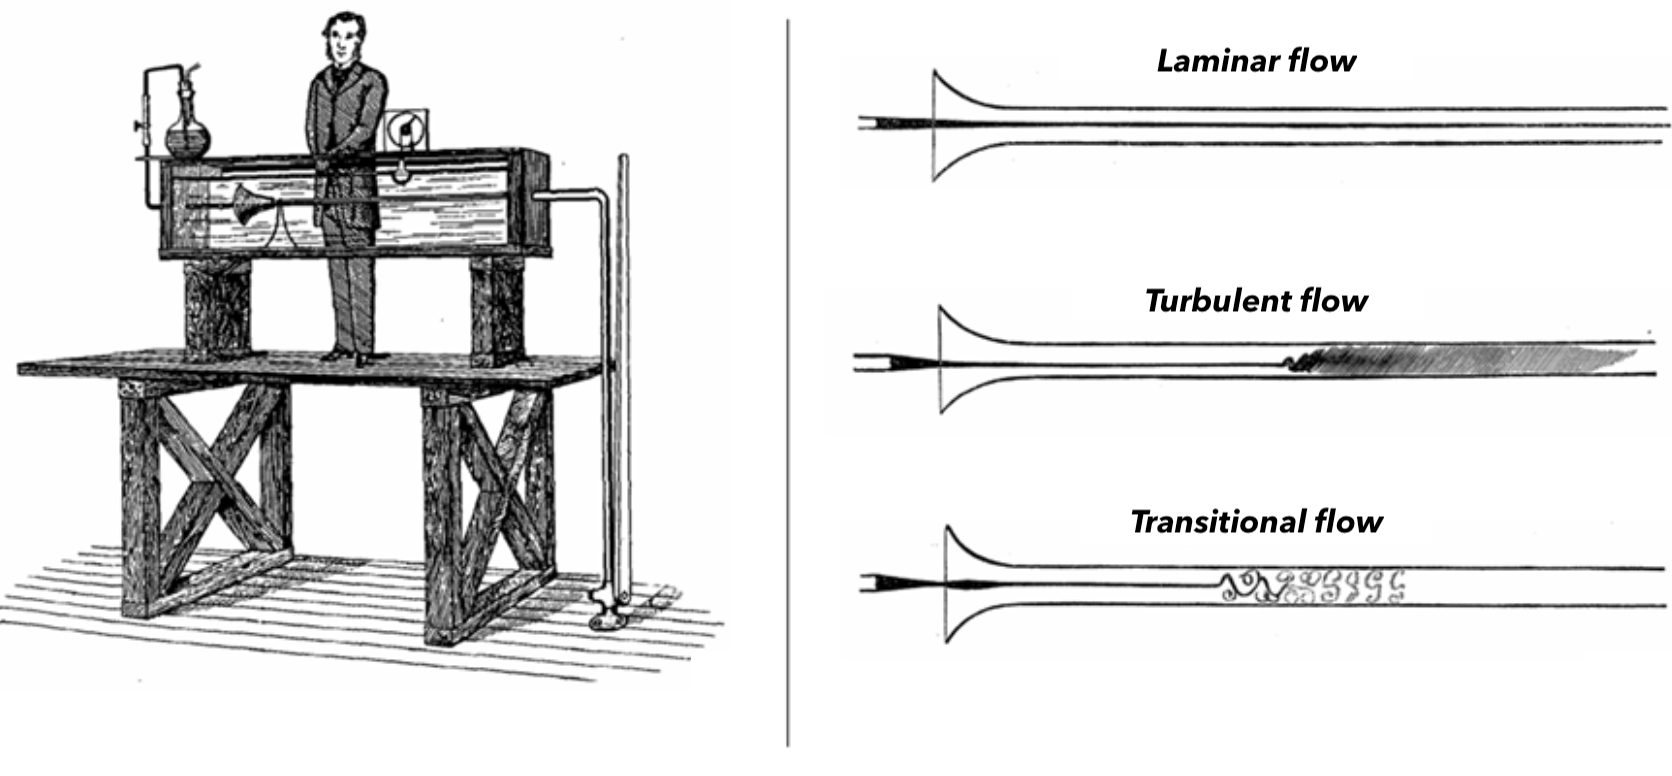
\includegraphics[width=1\textwidth]{grafici/reynolds_exp}
\caption{Sketch of the Reynolds experiment (\emph{left}) and flow patterns (\emph{right})}
\label{Reynolds:exp}
\end{center}
\end{figure}

with $u$ that is the characteristic velocity of the fluid, $l$ is the reference length of the scale and $\nu$ is the kinematic viscosity; able to predict the presence, or not, of the turbulence. He saw that when the inertia forces are huge the flow become unstable and the ink of its experiment started mixing with the surrounding water, as shown in the sketch of figure~\ref{Reynolds:exp}.
\par
This first work has correlated the presence of different states of the flow, laminar, transitional and turbulent, and their relationship with the couple viscous terms-nonlinear inertia term.
Further observations revealed the presence of three-dimensional eddies. Although we are still unable to determine their shapes, we have understood that they play a key role in the turbulence sustenance. Under the assumptions of incompressible flow, not subjected to external forces of volume or surface, the vorticity equation states
\begin{equation}
\frac{D \boldsymbol{\omega}}{D t} = (\boldsymbol{\omega} \cdot \boldsymbol{\nabla})\boldsymbol{u} + \nu \boldsymbol{\nabla}^{2} \boldsymbol{u}.
\end{equation}
Such equation, under a further simplification for inviscid flow, losses is rightmost term, remaining with only $ (\boldsymbol{\omega} \cdot \boldsymbol{\nabla})\boldsymbol{u}$, which determine the vortex-stretching. 
Vortex stretching is at the core of the description of the turbulence energy cascade from the large scales to the small scales in turbulence.
For incompressible flow, due to volume conservation of fluid elements, the lengthening implies thinning of the fluid elements in the directions perpendicular to the stretching direction. This reduces the length scale of the associated vorticity. Finally, at the smallest scales the turbulence kinetic energy is dissipated into heat through the action of molecular viscosity~\cite{Lumley}.


  


\subsection{Reynolds decomposition and time averaging}
The needing to employ a statistical approach require to express the quantities as a mean value plus fluctuations.\par
The expected value is calculated as a time averaged value and denoted with a bar, while the fluctuations with an appendix. Therefore we can express, for example the velocity, as
\begin{equation}
u(x,y,z,t) = \bar{u}(x,y,z) + u'(x,y,z,t).
\label{Reynolds:decomp}
\end{equation}
Two of the advantages of the Reynolds decomposition shown in equation~\ref{Reynolds:decomp} rely in the fact that the time average of the fluctuations is identically zero:
\begin{equation}
\frac{1}{T} \int_{0}^{T} u' dt =0,
\label{prop1}
\end{equation}
and the mean value is time-independent:
\begin{equation}
\frac{\partial \bar{u} }{\partial t} = 0
\label{prop2}
\end{equation}
\par
Since we have to deal with non-deterministic variables we have to define their ensemble average. In accordance with theory, an ensemble average owns a Gaussian probability distribution, thanks to the central limit theorem, so it can be no longer considered as a random variable. To be consistent with the theory we should perform $n$ times the same simulation under constant conditions.
However, in fluid dynamics, it is a common practice to exploit the ergodicity property of the processes, since, usually, the experiments are conducted under the assumption of stationary flow. 
Such property affirm that, since the process is stationary, the time averaged mean is equivalent to the ensemble average:
\begin{equation}
\langle p(\mathbf{x},t) \rangle = \frac{1}{T} \int_{0}^{T} p(\mathbf{x},t) dt.
\label{ergodic}
\end{equation}
When dealing with non-stationary processes, the equation~\ref{ergodic} is not fulfilled. Yet, this definition can still be considered valid if the sampling time $T$ is chosen small compared to the time needed for the average properties to change significantly.
\par
Expressing the Navier-Stokes equation using~\ref{Reynolds:decomp} and imposing a time averaging of the resulting equation, carrying out the simplifications due to~\ref{prop1} and~\ref{prop2}, the Reynolds averaged Navier-Stokes equation, or RANS, arise. Such equation is characterized by the appearance of a strongly non linear term, the viscous stresses term, which describe the turbulence.
\par
Although we have an equation capable of catching turbulence development using only averaged values we are still far from solving the problem. Unfortunately, the RANS equation, suffer the closure problem. We have to rely on turbulence models to evaluate the viscous, or Reynolds, stresses term. Thus we introduce an error, which is proportional to $\sqrt{u'u'}$, which is incompatible with our requirement to depict the turbulence with the highest level of fidelity possible.





\subsection{Elements of statistics}
Before introducing the concepts of correlations and spectral analysis, useful in our studies, we must define the probability density function and cumulative distribution function. \par
The cumulative distribution function is considered as the likelihood of an event to take place. It is a monotonically increasing curves and independently from its distribution it face the following properties:
\begin{equation*}
P(-\infty) = 0, \qquad P(+\infty) = 1 \qquad and \qquad \frac{\partial P(x)}{\partial x} = p(x)
\end{equation*}
where the latter term, $p(x)$, is the so called probability density function (PDF).
\par
The PDF is fundamental in the definition of the expected value
\begin{equation}
\langle u \rangle = \int_{-\infty}^{+\infty} u(x) p(x) dx
\end{equation}
and in the definition of the statistical moments
\begin{equation}
\sigma^{n} = \int_{-\infty}^{+\infty} (u(x) - \langle u \rangle)^{n} p(x)dx.
\label{statistic:momentum}
\end{equation}
Depending on the value of $n$, the equation~\ref{statistic:momentum} can define the variance ($n=2$), the skewness factor ($n=3$), the flatness factor ($n=4$) or higher statistical moments.
\par
When multiple variables are used we can recourse to the usage of the joined probability density function, $p_{x,y}(x,y)$. It exploit similar properties of the PDF and can be used to catch event characterized by the concomitancy. 
\par
It is particularly useful to determine the covariance of an event, defined as:
\begin{equation*}
\langle u_{1}u_{2} \rangle = \int_{-\infty}^{+\infty} \int_{-\infty}^{+\infty} \big( u_{1}(x_{1}) - \langle u_{1} \rangle \big) \big( u_{2}(x_{2}) - \langle u_{2} \rangle \big) p_{1,2}(x_{1},x_{2}) dx_{1} dx_{2}
\end{equation*}
\par
Starting from the result of the last equation we can define the correlation factor, $\rho_{1,2}$, as:
\begin{equation*}
\rho_{1,2} = \frac{\langle u_{1} u_{2} \rangle}{\sqrt{\langle u_{1}^{2} \rangle \langle u_{2}^{2} \rangle}}
\end{equation*}



\subsection{Correlations}

Keeping all the previous chapter definitions in mind and assuming ergodic processes, we can define the \emph{auto-covariance} factor as 
\begin{equation}
R_{uu}(\mathbf{x},\tau) = \langle u'(\mathbf{x},t) u'(\mathbf{x},t+\tau) \rangle
\label{autocovariance}
\end{equation}
The equation~\ref{autocovariance} represent the correlation between the signal from a given point in space at two different instants in time. \emph{Auto-covariance} gives an idea of the time needed by the signal itself to ``forget'' its past history, in a certain point in space. \par
The \emph{correlation coefficient} can be defined as:
\begin{equation*}
\rho(\tau) = \frac{R_{uu}(\mathbf{x},\tau)}{u_{rms}^{2}},
\end{equation*}
where $u_{rms}= \sqrt{\langle u'^{2} \rangle}$, which corresponds to $R_{uu}(\mathbf{x},0)$.\par

A similar definition could be provided to measure the correlation in space:
\begin{equation}
R_{ij}(\mathbf{x},\mathbf{r},t) = \langle u'(\mathbf{x},t) u'(\mathbf{x}+\mathbf{r},t) \rangle.
\label{covariance}
\end{equation}
The equation~\ref{covariance} represent the fluctuating parts of the velocity components correlation, set at distance $\mathbf{r}$, and it is called \emph{covariance}.\par
 



\subsection{Spectral analysis}
In the analysis of a random process, not all the necessary information can be deduced by its PDF. In the previous paragraph, correlation has proved to provide additional details about the relations established between different points in time and space. Introducing the spectral analysis enables the possibily to gain information about the energy distribution among the frequencies. In order to give a frequency description of turbulence to see which are the most energy containing frequencies, the Power Spectral Density has to be considered, and the tool used is the Fourier transform. Fourier introduced the idea to split the signal into different harmonics of different weight, in order to reproduce the signal itself. Hence, the signal domain experiences a shift, from time to frequency domain.
\begin{equation}
F(\omega) = \frac{1}{2\pi} \int_{-\infty}^{+\infty} e^{-i\omega t} f(t) dt.
\label{Fourier:t}
\end{equation}

Since the signals encountered when dealing with turbulence are continuous, a description of how the power is distributed between the different frequencies is useful. The power of a signal $u(t)$ is defined as:
\begin{equation}
P = \lim_{T \to \infty} \frac{1}{T} \int_{0}^{+\infty} u(t) dt.
\label{power:u}
\end{equation}
For numerous signals of interest, the equation~\ref{power:u} can not be casted in Fourier domain using~\ref{Fourier:t}. Therefore, the truncated Fourier transform is introduced:
\begin{equation*}
F_{T}(\omega) = \frac{1}{\sqrt{T}} \int_{0}^{+\infty} u(t) e^{i\omega t} dt.
\end{equation*}
The \emph{Power Spectral Density} can be therefore defined as:
\begin{equation*}
S_{uu} = \lim_{T\to \infty} \langle F_{T}(\omega) \rangle.
\end{equation*}
\par
One of the main interesting aspects of spectra analysis is that for a statistically stationary process, PSD constitutes the Fourier transform of the auto-covariance function $R(\mathbf{x},\tau)$:
\begin{equation*}
S_{uu} = \frac{1}{2\pi} \int_{-\infty}^{+\infty} R(\mathbf{x},\tau) e^{i\omega \tau} d\tau
\end{equation*}

and the anti Fourier transform

\begin{equation*}
R(\mathbf{x},\tau) = \int_{-\infty}^{+\infty} S_{uu} e^{i\omega t} d \omega.
\end{equation*}
\par
Since $u$ and $R(\mathbf{x},\tau)$ are both real-valued functions, their Fourier transform is an even function. Hence, $S_{uu}(\omega) = S_{uu}(-\omega)$. Here, a one-sided PSD in the positive frequency is considered
\begin{equation*}
P_{uu} = 2 S_{uu}(\omega)
\end{equation*}
If $\omega$ is positive, 0 otherwise.
\par
Frequently, it is preferred to compute the pre-multiplied one-dimensional energy spectra:
\begin{equation}
\Phi_{uu}^{+} = \frac{\alpha \Phi_{uu}}{u_{\tau}^{2}}
\label{psd}
\end{equation}
with $\Phi_{uu}$ the power spectral density of the streamwise velocity component, $\alpha$ is the streamwise wavenumber and $u_{\tau}$ the friction velocity. In this way, a more global view is allowed.
The same definition of~\ref{psd} applies also for the other two directions.




\subsection{Kolmogorov scales and viscous length scales}
In the previous sections we introduced the concept of scales. However, to completely understand the energy cascade process characteristic of turbulence, we have to define them properly.
\par
The large integral scales are the ones limited by the geometrical dimensions of the considered object. On the other hand the smallest scales are assumed to be independent of the outer geometrical restrictions and depend only on the viscosity and the viscous dissipation itself. They are referred to as the Kolmogorov scales and denoted as: length scale $\eta$, timescale $\tau_{\eta}$ and velocity scale $v_{\eta}$. 
\par
They are recovered through dimensional analysis, assuming independence among viscous dissipation $\epsilon$ and viscosity $\nu$, we can define the Kolmogorov scales as:
\begin{subequations}
\begin{align}
\eta = \sqrt[4]{ \frac{\nu^{3}}{\epsilon} }\\
\tau_{\eta} =\sqrt{ \frac{\nu}{\epsilon}}\\
u_{\eta} = \sqrt[4]{\nu \epsilon }
\end{align}
\end{subequations}

The energy cascade we talked few rows ago is the process which allows energy to transfer from the large sized scales, with their big whirls, to small scales. During such process the bigger whirls put in movement the flow, which generate smaller whirls and so on until the Kolmogorov microscales are reached. At such dimension the viscosity prevails against fluid motion, slowing it down and dissipating the energy through heat. \\~\par

Since close to the wall the main parameters of interest are the wall shear stress, $\tau_{w}$, and the kinematic viscosity, $\nu=\frac{\mu}{\rho}$, it is common practice to use values normalized on those quantities.\par
On this purpose we introduce the \emph{friction velocity} as:
\begin{equation*}
u_{\tau} = \sqrt{\frac{\tau_{w}}{\rho}},
\end{equation*}
and the \emph{viscous length scale} as:
\begin{equation*}
\delta_{\nu} = \frac{\nu}{u_{\tau}}
\end{equation*}
Combining them it is possible to define the $Re_{\tau}$ as:
\begin{equation*}
Re_{\tau} = \frac{u_{\tau}\delta_{\nu}}{\nu}
\end{equation*}
Starting from the definition of the \emph{viscous length scale} we can define the \emph{wall length scale}. \par
The \emph{wall length scale}, defined as
\begin{equation*}
y^{+} = \frac{y}{\delta_{\nu}},
\end{equation*}
is fundamental to determine the turbulence layers. Those layers divide the near wall regions, based on turbulence generation mechanism.
Starting from the wall, we find:
\begin{itemize}
\item the \emph{viscous sublayer} $(y^{+}<5)$, here the entire generation mechanism rely exclusively on viscous effects;
\item the \emph{buffer layer} $(5<y^{+}<30)$, where the turbulence generation is due to the overlapping effects of viscosity and Reynolds stresses;
\item the \emph{log-law region} $(30<y^{+}<0.1y)$, in this region we face the arise of the homonym law, that will be discussed later in detail;
\item the \emph{outer-layer} $(y^{+}>50)$, in this region the Reynolds stresses moves the turbulence engine.
\end{itemize}


  